\documentclass[aspectratio=169]{beamer}

\usepackage{global-macros}
\usepackage{graphicx}
\graphicspath{{../fig}}
\usepackage{algpseudocode, algorithm}
\usepackage{biblatex}

\vfuzz=30pt


\addbibresource{../bib/bibliography.bib}

\title{NPIV estimation through functional SGD}
\author{Student: Caio Lins
        \\ Advisor: Yuri Saporito
}
\institute{EMAp -- FGV}
\date{\today}

\titlegraphic{
    
\includegraphics[width=3cm]{logo.png}
}

\AtBeginSection[]
{%
  \begin{frame}
    \frametitle{Summary}
    \tableofcontents[currentsection]
  \end{frame}
}

\addtobeamertemplate{navigation symbols}{}{%
    \usebeamerfont{footline}%
    \usebeamercolor[fg]{footline}%
    \hspace{1em}%
    \insertframenumber/\inserttotalframenumber
}

\newcommand{\boldf}{\boldsymbol{f}}

\newcommand{\hstar}{h^{ \star }}
\newcommand{\risk}{\mathcal{R}}
\newcommand{\loss}{\ell}
\renewcommand{\hat}{\widehat}
\newcommand{\iid}{\overset{\mathrm{iid}}{\sim}}
\DeclareMathOperator{\diam}{diam}
\newcommand{\data}{\mathcal{D}}
\newcommand{\dataproj}{\mathcal{D}_{ \mathrm{proj} }}


\begin{document}

    \frame{\titlepage}

    \section{NPIV estimation}

    \begin{frame}{Instrumental Variables}
        \begin{itemize}
            \item<1-> Consider a generic regression problem:
                \begin{equation*}
                    Y = \hstar ( X ) + \varepsilon
                ,\end{equation*}
                where $ \mean [ \varepsilon ] = 0 $ and we wish to estimate $ h^{ \star } $.

                \item<2-> What happens if $ \varepsilon \not\kern-1pt\indep X $? That is, $ \mean [ \varepsilon \mid X ] \neq 0 $?
                \item<3-> Minimizing $ \mean [ ( Y - h ( X ) )^2 ] $ over $ h $ gives biased results.
                \uncover<4->{
                    \begin{equation*}
                        Y = \underbrace{ \hstar ( X ) + \mean [ \varepsilon \mid X ] }_{ = \ f ( X )\text{ for some $ f $ } } + ( \varepsilon - \mean [ \varepsilon \mid X ] )
                    .\end{equation*}
                }
                \item<5-> We end up estimating $ f $ instead of $ \hstar $!
        \end{itemize}
    \end{frame}

    \begin{frame}{Instrumental Variable}
        \begin{itemize}
            \item<1-> Suppose we have access to a variable $ Z $ such that
                \begin{enumerate}
                    \item<2-> $ Z \not\kern-1pt\indep X $, i.e., $ \mean [ X \mid Z ] $ is not constant,
                    \item<3-> $ Z $ affects $ Y $ only through $ X $,
                    \item<4-> $ \varepsilon \indep Z $, i.e., $ \mean [ \varepsilon \mid Z ] = 0 $.
                \end{enumerate}
                \uncover<5->{$ Z $ is called an \emph{instrumental variable}.}
                \item<6-> How does it help us?
        \end{itemize}
    \end{frame}

    \begin{frame}{Instrumental Variable}
       \begin{itemize}
           \item<1->  Structural equation:
               \begin{equation*}
                   Y = \hstar ( X ) + \varepsilon
               ,\end{equation*}
               where $ \mean [ \varepsilon \mid Z ] = 0 $.
           \item<2-> Consider minimizing $ \risk ( h ) = \mean \left[ \left( \mean [ Y - h ( X ) \mid Z ] \right)^2 \right] $ over $ h $.
            \item<3-> Since
                \begin{equation*}
                    \mean [ Y \mid Z ] = \mean [ \hstar ( X ) + \varepsilon \mid Z ] = \mean [ \hstar ( X ) \mid Z ]
                ,\end{equation*}
                \uncover<4->{
                    We have
                    \begin{equation*}
                        \risk ( h ) = \mean \left[
                            \left(
                                \mean \left[
                                    ( \hstar - h ) ( X )
                                    \mid Z
                                \right]
                            \right)^2
                        \right]
                    .\end{equation*}
                }
                \item<5-> $ \risk ( h ) = 0 \iff \mean \left[ \left( \hstar - h \right) ( X ) \mid Z \right] = 0 \iff \mean [ \hstar ( X ) \mid Z ] = \mean [ h ( X ) \mid Z ] $.
                \item<6-> Still does \emph{not} imply $ h = \hstar $, but reduces bias \emph{if $ Z $ is a good instrument}.
       \end{itemize} 
    \end{frame}

    \begin{frame}{Example}
        \begin{equation*}
            \underbrace{\text{Grades}}_{Y} = \hstar \bigl( \underbrace{ \text{Attends tutoring sessions?} }_{X} \bigr) + \varepsilon
        .\end{equation*}
        \begin{itemize}
            \item<2-> Natural ability is a confounding variable: maybe only people who struggle a lot go to tutoring sessions.
            \item<3-> $ Z = \text{Lives close to school?} $
                \begin{enumerate}
                    \item<4-> $ Z \not\kern-1pt\indep X $,
                    \item<4-> $ Z $ affects $ Y $ only through $ X $, \uncover<5->{{\color{red}(Kind of)}}
                    \item<4-> $ \varepsilon \indep $ Z $ $.
                \end{enumerate}
        \end{itemize}
    \end{frame}

    \begin{frame}{NPIV estimation}
        \begin{itemize}
            \item<1-> Stands for ``Nonparametric Instrumental Variable estimation''.
            \item<2-> No assumptions on some parametric form for $ \hstar $.
        \end{itemize}
    \end{frame}

    \section{Our approach}

    % Stochastic gradient computation
    % Pseudo algorithm

    \begin{frame}{Problem formulation}
        \begin{itemize}
            \item<1-> We have
                \begin{equation*}
                    Y = \hstar ( X ) + \varepsilon   
                ,\end{equation*}
                 where $ \mean [ \varepsilon \mid Z ] = 0 $, and want to estimate $ \hstar $.
            \item<2-> Equivalently,
                \begin{equation*}
                    r_{ 0 } ( Z ) = \mathcal{T} [ \hstar ] ( Z )   
                ,\end{equation*}
                with
                \begin{itemize}
                    \item<3-> $ r_{ 0 } ( Z ) = \mean [ Y \mid Z ] $,
                    \item<3-> $ \mathcal{T} [ h ] ( Z ) = \mean [ h ( X ) \mid Z ] $.
                \end{itemize}
            \item<4-> Risk measure:
                \begin{equation*}
                    \risk ( h ) = \mean \left[ \frac{ 1 }{ 2 } \left( \mean \left[ Y - h ( X ) \mid Z \right] \right)^2 \right] = \mean \left[ \frac{ 1 }{ 2 } \left( r_{ 0 } ( Z ) - \mathcal{T} [ h ] ( Z ) \right)^2 \right]
                .\end{equation*}
        \end{itemize}
    \end{frame}

    \begin{frame}{Stochastic Gradients}
        \begin{itemize}
            \item<1-> It turns out that $ \nabla \risk ( h ) ( X ) = \mathcal{T}^{ * } [ \mathcal{T} [ h ] - r_{ 0 } ] ( X ) $.
            \item<2-> Immediate idea:
                \begin{equation*}
                    \begin{cases}
                        h_{ 0 } \equiv 0, \\
                        h_{ t } \leftarrow h_{ t-1 } - \alpha_{ t } \nabla \risk ( h_{ t-1 } ) \quad \text{for} $ t \geq 1 $.
                    \end{cases}
                \end{equation*}
        \end{itemize}
    \end{frame}

    \begin{frame}{Stochastic Gradients}
        \begin{itemize}
            \item<1-> Problem: \emph{We don't observe} $ r_{ 0 } $ \emph{neither know how to compute}  $ \mathcal{T}^{ * } $ \emph{nor} $ \mathcal{T} $.
                \uncover<2->{We only have access to joint independent samples from $ X, Y $ and $ Z $.}
            \item<3-> Solution 1: ``No problem, we estimate everything!'' \uncover<2->{\dots doable, but horrible, since $ \mathcal{T}^{ * } [ \mathcal{T} [ h ] - r_{ 0 } ] $ involves plugin estimates into other estimates.
                Goodbye theoretical guarantees.}
        \end{itemize}
    \end{frame}

    \begin{frame}{Stochastic Gradients}
        \begin{itemize}
            \item<1-> Solution 2: Notice that
                \begin{equation*}
                    \nabla \risk ( h ) ( X ) = \mean_{ Z } \left[ \Phi ( X, Z ) ( \mathcal{T} [ h ] ( Z ) - r_{ 0 } ( Z ) ) \right]
                ,\end{equation*}
                where $ \Phi ( x, z ) = \frac{ p ( x, z ) }{ p ( x ) p ( z ) } $.
            \item<2-> Second idea: \emph{Now} we estimate everything:
                    \begin{equation*}
                        \begin{cases}
                            h_{ 0 } \equiv 0, \\
                            h_{ t } \leftarrow \hat{ \Phi } ( \cdot, Z_{ i } ) \left( \hat{ \mathcal{T} [ h_{ t-1 } ] } ( Z_{ i } ) - \hat{ r_{ 0 } } ( Z_{ i } ) \right).
                        \end{cases}
                    \end{equation*}
                \item<3-> \dots Not pretty, but manageable, since we no longer have iterated conditional expectations \uncover<4->{\color{red}(but must estimate ratio of densities)}.
        \end{itemize}
    \end{frame}

    \section{Where we are at}

    \begin{frame}{Prototype}
        Prototype gave reasonable results
        \begin{figure}[htb]
            \begin{center}
                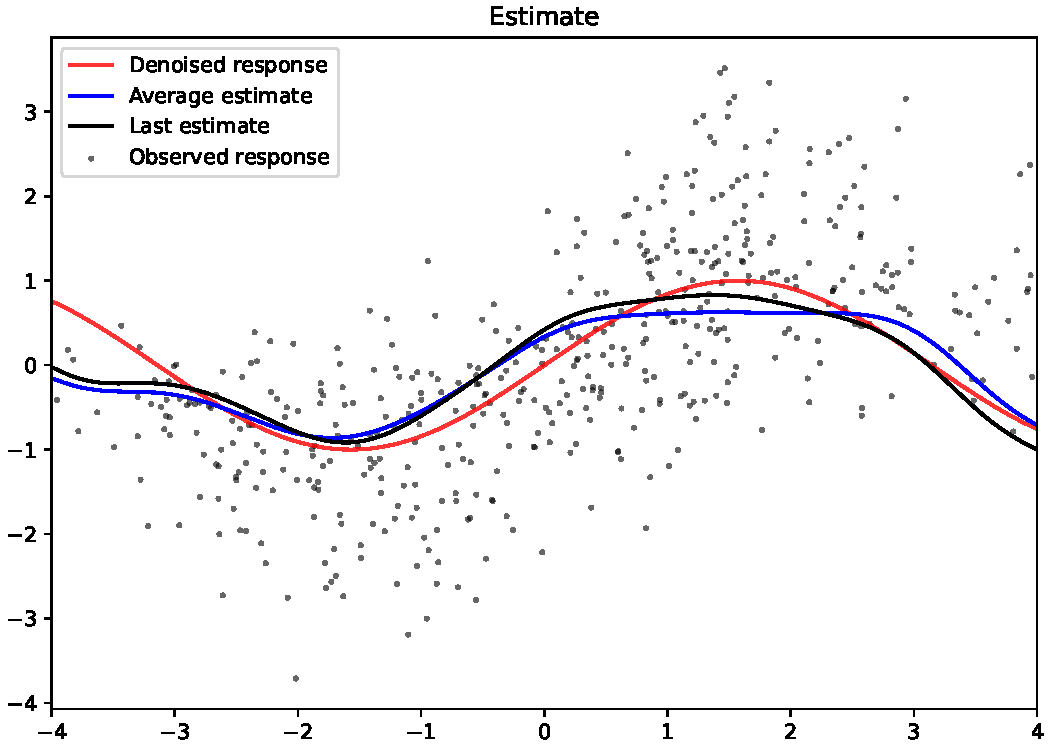
\includegraphics[width=.5\textwidth]{estimate.pdf}
                \caption{In red we have $ \hstar = \sin $, in black we have $ h_{ N } $ and in blue, $ \frac{ 1 }{ N } \sum_{ t=1 }^{ N } h_{ N } $.}
                \label{fig: prototype}
            \end{center}
        \end{figure}
    \end{frame}

    \begin{frame}{Theoretical properties}
        \begin{itemize}
            \item<1-> Still working on convergence guarantees.
            \item<2-> This is helping us find better ways to estimate $ \Phi $ and $ \mathcal{T} $ (mainly RKHS methods).
        \end{itemize}
    \end{frame}

    \section{Next steps}

    \begin{frame}{Next steps}
        \begin{itemize}
            \item<1-> Finalize convergence guarantees.
            \item<2-> Implement modifications which the theory points to.
            \item<3-> Benchmark against current methods.
        \end{itemize}
    \end{frame}

    \begin{frame}
        \frametitle{References}
        \nocite{*}
        \printbibliography
    \end{frame}

    \begin{frame}
        \centering Thank You!
    \end{frame}

\end{document}
